\chapter{Day 1: Facial Recognition: The Big Picture}

\section{Schedule}
\begin{itemize}
\item 0900-0920: Welcome - A letter to my future self
\item 0920-0950: A simple face detection: Round 1
\item 0950-1010: Round 2: What did you notice?
\item 1010-1030: Debrief: What did we learn?
\item 1030-1045: Coffee
\item 1045-1055: Pixel arithmetic
\item 1055-1105: A Universal Set of Building Blocks
\item 1105-1125: A Better Set of Building Blocks?
\item 1125-1145: Towards an Optimal Basis
\item 1145-1200: Broadcast debrief (via Zoom)
\item 1200-1220: Course logistics 
\item 1220-1230: Day 1 survey
\end{itemize}

Welcome to QEA Module One! In this module, you will develop software to recognize your face among everyone in QEA (hello, new late-night security). It all functions through applying some beautiful mathematics and using computational tools. Let's first imagine how a computer ``sees" an image as numbers. 

\section{Facial recognition- "seeing" via numbers} 

\subsection{Round 1: From images to numbers [30 mins]}
At your table you will find a smiley face. Imagine converting this face into a form that a computer can understand (i.e., numbers). A grid is superimposed on the face for your reference. 

\paragraph{Goal}Design a method that enables a "computer" to (approximately) reproduce the face from a list of numbers and an algorithm that you define. The numbers can be grouped within the list, but your list should contain numbers only. An example of a group of numbers is [2,4] or [0, 100, 14]. You will create the algorithm (or, equivalently, the instructions) that tell the computer what to do with your list of numbers. 

When you've defined your group's method, 
\begin{itemize}
    \item Generate the list of numbers that represents your face using your method. 
    \item Make a set of instructions (your "algorithm") on your portable white board using a BLACK marker so that another group can recreate your image from your list of numbers.  
    \item Trade instructions with another group.
    \item Create the other group's face from their algorithm on the blank grid. 
    \item Record any challenges you encounter on their portable whiteboard using a RED marker.
    \item Exchange back your original materials and debrief on what you've learned about your method at your table. 
\end{itemize}

\subsection{Round 2 [20 mins]}
\paragraph{Goal}Adjust your method to be able to distinguish the new faces that you've just been given.  The 8x8 grid is shown for reference; you are not restricted to this grid. 

Discuss the following and record your answers on your portable whiteboard:
\begin{itemize}
    \item How does your method need to transform the original image in order to "see" the detail of the  face?
    \item What "demands" does your new method make on the computer compared to the old method?  (Remember that the computer is using your algorithm and numbers to represent the images) 
    \item Consider a photo of a human face, in what ways does your numerical method contain inherent limits or biases? 
\end{itemize}

\subsection{A debrief (in each room) [20 mins]}

\subsection{Coffee Break [15 min]}

\section{Facespace}

Before the coffee break we thought about various ways to represent an image (e.g., a picture of a face).  In this section we're going to narrow in on a particular method of representing images: as a weighted sum of a set of building block images.  In this section you'll work through some exercises to scaffold the basic ideas of how this type of representation works and why it is so powerful.

\subsection{Pixel Arithmetic [10 mins]}
Adding is one of the most basic operations in mathematics.  While everyone here is familiar with the concept of adding numbers, we can generalize this idea to add together other sorts of entities.  We can even think about what it means to add two images together.

As a simple example, let's add the following two images together (we'll explain more precisely how we are defining addition of images once you've seen the result).
\begin{align}
\begin{tabular}{|c|c|c|c|c|c|c|c|c|c|c|}
\hline
 &   &  &  & & & & & & & \\
 \hline
&    &   & \cellcolor{black}   & \cellcolor{black}   & \cellcolor{black}   & \cellcolor{black}  & \cellcolor{black}  & & & \\
 \hline
 &   &  \cellcolor{black} & & & & & & \cellcolor{black} & &    \\
 \hline
  &   \cellcolor{black} & & & & & & & & \cellcolor{black} &    \\
   \hline
    &   \cellcolor{black} & & & & & & & & \cellcolor{black} &    \\
     \hline
  &   \cellcolor{black} & & & & & & & & \cellcolor{black} &    \\
 \hline
  &   \cellcolor{black} & & & & & & & & \cellcolor{black} &    \\
   \hline
  &   \cellcolor{black} & & & & & & & & \cellcolor{black} &    \\
\hline
 &   &  \cellcolor{black} & & & & & & \cellcolor{black} & &    \\
 \hline
 &    &   & \cellcolor{black}   & \cellcolor{black}   & \cellcolor{black}   & \cellcolor{black}  & \cellcolor{black}  & & & \\
\hline
 &   &  &  & & & & & & & \\
 \hline
\end{tabular} ~+~& 
\begin{tabular}{|c|c|c|c|c|c|c|c|c|c|c|}
\hline
 &   &  &  & & & & & & & \\
 \hline
 &   &  &  & & & & & & & \\
 \hline
 &   &  &  & & & & & & & \\
 \hline
 &   &  &  & & & & & & & \\
   \hline
    &  & & & \cellcolor{black} & & \cellcolor{black}& & & &    \\
     \hline
 &   &  &  & & & & & & & \\
 \hline
  &  & &\cellcolor{black}  & & & & \cellcolor{black} & & &    \\
   \hline
  &  & & & \cellcolor{black} & \cellcolor{black}  & \cellcolor{black} & & & &    \\
\hline
 &   &  &  & & & & & & & \\
 \hline
 &   &  &  & & & & & & & \\
\hline
 &   &  &  & & & & & & & \\
 \hline
\end{tabular} \nonumber \\
=~&\begin{tabular}{|c|c|c|c|c|c|c|c|c|c|c|}
\hline
 &   &  &  & & & & & & & \\
 \hline
&    &   & \cellcolor{black}   & \cellcolor{black}   & \cellcolor{black}   & \cellcolor{black}  & \cellcolor{black}  & & & \\
 \hline
 &   &  \cellcolor{black} & & & & & & \cellcolor{black} & &    \\
 \hline
  &   \cellcolor{black} & & & & & & & & \cellcolor{black} &    \\
   \hline
    &   \cellcolor{black} & & & \cellcolor{black} & & \cellcolor{black}& & & \cellcolor{black} &    \\
     \hline
  &   \cellcolor{black} & & & & & & & & \cellcolor{black} &    \\
 \hline
  &   \cellcolor{black} & &\cellcolor{black}  & & & & \cellcolor{black} & & \cellcolor{black} &    \\
   \hline
  &   \cellcolor{black} & & & \cellcolor{black} & \cellcolor{black}  & \cellcolor{black} & & & \cellcolor{black} &    \\
\hline
 &   &  \cellcolor{black} & & & & & & \cellcolor{black} & &    \\
 \hline
 &    &   & \cellcolor{black}   & \cellcolor{black}   & \cellcolor{black}   & \cellcolor{black}  & \cellcolor{black}  & & & \\
\hline
 &   &  &  & & & & & & & \\
 \hline
\end{tabular} \nonumber 
\end{align}

Conceptually, this operation might seem straightforward.  Adding two images results in an image that has a black pixel whenever either of the two images has a black pixel at a corresponding position.

More formally, we can think about black pixels as having a value of 255 and white pixels as having a value of 0 (gray pixels would have a value between these two values depending on how dark they are). (A scale from 0 to 255 seems like a weird choice, but there is a very good reason why this is the standard - remember that digital storage uses binary (bit) - how many integers can you represent with an 8-bit number?)  To add two images together, all we do is add the corresponding elements at a particular point in the grid!  In this way addition on images works much the same as addition of a single number--the only difference is we perform the addition of single numbers multiple times for each position in the grid.

\tcbset{colback=white}
\begin{prob}
With your tablemates, work through the following pixel arithmetic problems on the board.
\begin{enumerate}
\item
\begin{align}
\begin{tabular}{|c|c|c|}
\hline
\cellcolor{black}& & \\
\hline
& \cellcolor{black} & \\
\hline
& & \cellcolor{black} \\
\hline
\end{tabular} + \begin{tabular}{|c|c|c|}
\hline
 & &\cellcolor{black} \\
\hline
& & \\
\hline
 \cellcolor{black} & & \\
\hline
\end{tabular}\nonumber
\end{align}

\item

\begin{align}
\begin{tabular}{|c|c|c|}
\hline
\cellcolor{black}& & \\
\hline
& \cellcolor{gray} & \\
\hline
& & \cellcolor{black} \\
\hline
\end{tabular} + \begin{tabular}{|c|c|c|}
\hline
 & &\cellcolor{black} \\
\hline
& \cellcolor{gray} & \\
\hline
 \cellcolor{black} & & \\
\hline
\end{tabular}\nonumber
\end{align}
\end{enumerate}
\end{prob}

Without too much of a leap, we can also multiply images by a number by simply multiplying each element in the image by that value.  We can think of this multiplication operation as ``scaling'' the image.

For example, 

\begin{align}
0.5 \times \begin{tabular}{|c|c|c|}
\hline
& &\cellcolor{black} \\
\hline
& \cellcolor{black} & \\
\hline
 \cellcolor{black}& & \\
\hline
\end{tabular} = \begin{tabular}{|c|c|c|}
\hline
 & &\cellcolor{gray} \\
\hline
& \cellcolor{gray} & \\
\hline
 \cellcolor{gray} & & \\
\hline
\end{tabular}\nonumber
\end{align}

\begin{prob}
With your tablemates, work through the following pixel arithmetic problems on the board.
\begin{enumerate}
\item

\begin{align}
0.5 \times \begin{tabular}{|c|c|c|}
\hline
\cellcolor{black}& & \\
\hline
& \cellcolor{gray} & \\
\hline
& & \cellcolor{black} \\
\hline
\end{tabular} + 0.5 \times \begin{tabular}{|c|c|c|}
\hline
\cellcolor{black} & & \\
\hline
& \cellcolor{gray} & \\
\hline
& & \cellcolor{black} \\
\hline
\end{tabular} \nonumber
\end{align}

\item \begin{align}
0.5 \times \begin{tabular}{|c|c|c|}
\hline
\cellcolor{black}& & \\
\hline
& \cellcolor{gray} & \\
\hline
& & \cellcolor{black} \\
\hline
\end{tabular} + 0.5 \times \begin{tabular}{|c|c|c|}
\hline
 & &\cellcolor{black} \\
\hline
& \cellcolor{gray} & \\
\hline
 \cellcolor{black} & & \\
\hline
\end{tabular}\nonumber
\end{align}

\item (Don't think about this one too hard.  Just draw approximately what this would be) \begin{align}
0.9999 \times \begin{tabular}{|c|c|c|}
\hline
\cellcolor{black}& & \\
\hline
& \cellcolor{gray} & \\
\hline
& & \cellcolor{black} \\
\hline
\end{tabular} + 0.0001 \times \begin{tabular}{|c|c|c|}
\hline
 & &\cellcolor{black} \\
\hline
& \cellcolor{gray} & \\
\hline
 \cellcolor{black} & & \\
\hline
\end{tabular}\nonumber
\end{align}
\end{enumerate}
\end{prob}

\subsection{A Universal Set of Building Block Images [10 mins]}

Now that we have a sense of how we can add and scale images, let's think about how we might construct a set of building block images such that we can construct any image as a sum of scaled versions of these building blocks.

\begin{prob}
With your tablemates, work through the following problems.
\begin{enumerate}
\item What is the range of images that could be constructed by summing over scaled versions of the following building block images? ($c$ is a number between 0 and 1).  Another way to think about this is, as you sweep the value of $c$ from 0 to 1, how does the resultant sum of the two images change?
 \begin{align}
c \times \begin{tabular}{|c|c|c|}
\hline
\cellcolor{black}& & \\
\hline
& \cellcolor{black} & \\
\hline
& & \cellcolor{black} \\
\hline
\end{tabular} + (1-c) \times \begin{tabular}{|c|c|c|}
\hline
 & &\cellcolor{black} \\
\hline
& \cellcolor{black} & \\
\hline
 \cellcolor{black} & & \\
\hline
\end{tabular}\nonumber
\end{align}
\item What is the range of images that could be constructed by summing over scaled versions of the following building block images? ($a$ and $b$ are both numbers between 0 and 1).  Instead of having one knob to turn (as in the previous exercise), you now have two.

\begin{align}
a~\begin{tabular}{|c|c|c|c|c|c|c|c|c|c|c|}
\hline
 &   &  &  & & & & & & & \\
 \hline
&    &   & \cellcolor{black}   & \cellcolor{black}   & \cellcolor{black}   & \cellcolor{black}  & \cellcolor{black}  & & & \\
 \hline
 &   &  \cellcolor{black} & & & & & & \cellcolor{black} & &    \\
 \hline
  &   \cellcolor{black} & & & & & & & & \cellcolor{black} &    \\
   \hline
    &   \cellcolor{black} & & & & & & & & \cellcolor{black} &    \\
     \hline
  &   \cellcolor{black} & & & & & & & & \cellcolor{black} &    \\
 \hline
  &   \cellcolor{black} & & & & & & & & \cellcolor{black} &    \\
   \hline
  &   \cellcolor{black} & & & & & & & & \cellcolor{black} &    \\
\hline
 &   &  \cellcolor{black} & & & & & & \cellcolor{black} & &    \\
 \hline
 &    &   & \cellcolor{black}   & \cellcolor{black}   & \cellcolor{black}   & \cellcolor{black}  & \cellcolor{black}  & & & \\
\hline
 &   &  &  & & & & & & & \\
 \hline
\end{tabular} ~+~b~& 
\begin{tabular}{|c|c|c|c|c|c|c|c|c|c|c|}
\hline
 &   &  &  & & & & & & & \\
 \hline
 &   &  &  & & & & & & & \\
 \hline
 &   &  &  & & & & & & & \\
 \hline
 &   &  &  & & & & & & & \\
   \hline
    &  & & & \cellcolor{black} & & \cellcolor{black}& & & &    \\
     \hline
 &   &  &  & & & & & & & \\
 \hline
  &  & &\cellcolor{black}  & & & & \cellcolor{black} & & &    \\
   \hline
  &  & & & \cellcolor{black} & \cellcolor{black}  & \cellcolor{black} & & & &    \\
\hline
 &   &  &  & & & & & & & \\
 \hline
 &   &  &  & & & & & & & \\
\hline
 &   &  &  & & & & & & & \\
 \hline
\end{tabular} \nonumber
\end{align}

In this case we can think of the values $a$ and $b$ as encoding of a particular smiley face.  You will deduce the effect that both $a$ and $b$ have on the specific nature of the smiley face.

\item Building on the previous example, come up with your own way of representing a simple face like the one above as the sum of two or more scaled building block images.  This is intended to be fun, so be creative!  It's up to you what sort of faces that your method is capable of representing.

\item You probably noticed from the previous three exercises that not all possible images can be constructed by adding scaled versions from a small set of building block images.  Suppose you wanted to be able to represent \emph{any} possible 3 pixel by 3 pixel image of a face.  While there are many possible ways to do this, for simplicity each of your building block images should only have a single black pixel (the rest should be white).  At the board, define a set of building block images that lets you represent any possible 3 pixel by 3 pixel face in this manner.  How many building block images did you need to represent all possible 3 pixel by 3 pixel faces?  Are there any images that can't be represented as a sum of scaled versions from your building block images?  How many building block images would you need if you wanted to encode all possible 5 pixel by 5 pixel faces?  What about n pixels by n pixels?  

\end{enumerate}
\end{prob}
\tcbset{colback=black!5!white}

\subsection{A Better Set of Building Blocks? [20 mins]}

At the end of the previous section you showed how can represent any possible image as a sum of scaled single-pixel images.  This is a very powerful idea, but we can take it even farther.  Before we continue, let's think about some of the ways in which this way of representing face images is not so great.

\begin{prob}
Suppose you wish to represent 19 pixel by 19 pixel images of faces using the scheme you devised in the previous set of exercises (as a sum of scaled, single-pixel images).  Here is an example of what such a face might look like.
\begin{center}
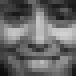
\includegraphics[width=0.2\linewidth]{FacesDay1/figs/face0400}
\end{center}

\begin{enumerate}
\item If you think of the representation of each image as the scaling factor that you apply to each of your single-pixel images, how many numbers do you need to specify this one face image (you answered almost this exact question in the previous part, so don't overthink this).
\item How many numbers would you need to represent a 19 pixel by 19 pixel image of a flower?  How many numbers would you need to represent a completely random 19 pixel by 19 images (one with no special structure)?
\item Suppose someone gives you one of the numbers needed to encode a particular face?  Without looking at the face image itself, how much information (e.g., age, identity, sex, gender, etc.) could you determine about the face just from that one number?
\end{enumerate}
\end{prob}

As you probably deduced in the previous exercise, a major drawback of the encoding we worked out previously is that each scaling factor doesn't really tell us that much useful information about each face (and as a result we need a lot of these numbers to specify a particular face).  It turns out that we can fix a lot of these shortcomings through more carefully choosing our set of building block images.  Reframing problems by choosing a different set of building blocks is going to be one of the key ideas in this module.

Come to the front of the room and grab a piece of paper with a 6 by 4 grid of face-like images along with a set of transparent face-like images held by a binder clip.  Take these materials back to your table.  Layout the piece of paper on your table.  Also in the envelope you should have a set of transparent versions of those same building block images.  Layout the transparent building block images so that they align with the appropriate printed building block image.  The bottom building block should go in the upper left corner of the printed sheet.  As a sanity check, make sure the textured side of the transparency is facing up (one side will be smooth and the other textured).  Be very careful when laying out your images as it is hard to get them back in the right order.

What you see before you is a very carefully chosen set of building block images.  You should notice that each row represents a different building block image and each column represents a different scaled version of that same building block.  Today, we won't be going into detail about \emph{how} we determined these particular building blocks but we will be having you experiment with them in order to understand, at a conceptual level, some of their properties.

\begin{itemize}
\item You can add these scaled building block images by simply stacking multiple transparencies on top of each other and placing them on a white background (make sure to keep them aligned).  We've found that using your thumb and index finger and pinching the middle of the transparency is a good way to pick it up (they are pretty sturdy).
\item Along with these building block images, we have determined optimal encodings for a bunch of different faces.  At your table, pick a few of these faces and try assembling them (you should probably put the transparencies back after assembling each face so you can keep better track of the transparencies).

\emph{Note: that each column in the table corresponds to one of the building block images (row of your transparencies).  Higher numbers in the table correspond to choosing the darker (more saturated) versions of each building block image.  If a 0 appears for a particular building block, don't include that building block at all to construct a particular face.}

\small{
\begin{longtable}{c|c|c|c|c|c|c}
\textbf{Intensity 1} & \textbf{Intensity 2}  & \textbf{Intensity 3}  &  \textbf{Intensity 4} & \textbf{Intensity 5}&  \textbf{Intensity 6} & \textbf{face image} \\
\hline
3 & 3 & 0 & 0 & 2 & 2 &  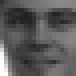
\includegraphics{FacesDay1/figs/face0015.png} \\
\hline
0 & 2 & 3 & 2 & 3 & 1 &   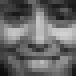
\includegraphics{FacesDay1/figs/face0400.png} \\
\hline
3 & 0 & 1 & 4 & 1 & 1 & 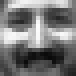
\includegraphics{FacesDay1/figs/face1000.png} \\
\hline
1 & 4 & 1 & 2 & 3 & 4 &  
\includegraphics{FacesDay1/figs/face0600.png} \\
\hline
0 & 0 & 3 & 3 & 2 & 1 &  
\includegraphics{FacesDay1/figs/face2300.png} \\
\hline
2 & 0 & 3 & 0 & 2 & 0 &  
\includegraphics{FacesDay1/figs/face1030.png} \\
\hline
2 & 0 & 1 & 3 & 0 & 1 &  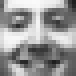
\includegraphics{FacesDay1/figs/face1270.png} \\
\hline
1& 2& 0 & 1 &0 & 0 &  
\includegraphics{FacesDay1/figs/face1180.png} \\
\hline
1& 1& 3 & 0 & 1 & 2 &  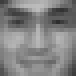
\includegraphics{FacesDay1/figs/face1260.png} \\
\hline
2 & 0 & 1 & 3 & 0 & 1 &  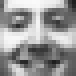
\includegraphics{FacesDay1/figs/face1270.png} \\
\hline
3 & 2 & 0 & 2 & 0 & 1 &  
\includegraphics{FacesDay1/figs/face0960.png}  \\
\hline
2 & 1 & 3 & 0 & 3 & 1 &  
\includegraphics{FacesDay1/figs/face0160.png}  \\
\hline
0 & 3 & 0 & 1 & 3 & 3 &  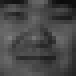
\includegraphics{FacesDay1/figs/face0615.png}  \\
\hline
2 & 3 & 0 & 1 & 2 & 1 &  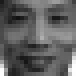
\includegraphics{FacesDay1/figs/face0250.png} 
\end{longtable}}
\normalsize
\item How many numbers do you now need to encode a 19 pixel by 19 pixel face?
\item Can you encode any possible face with this set of building blocks?
\item How well does this set of building blocks work for encoding these faces?  Does it seem to work equally well across all faces?  Which faces does it work well on (i.e., they can accurately be reconstructed from the building blocks) and which faces does it work poorly on?
\item Looking at the building blocks themselves, what does each building block seem to represent?  In other words, as you increases the amount of a particular building block, what features or qualities does that impart on the resulting face.  To help you think this through, below we have a grid of faces where each row corresponds with one of the six building block images and each of the faces in the row contains a large amount of that particular building block image in its encoding.

\begin{center}
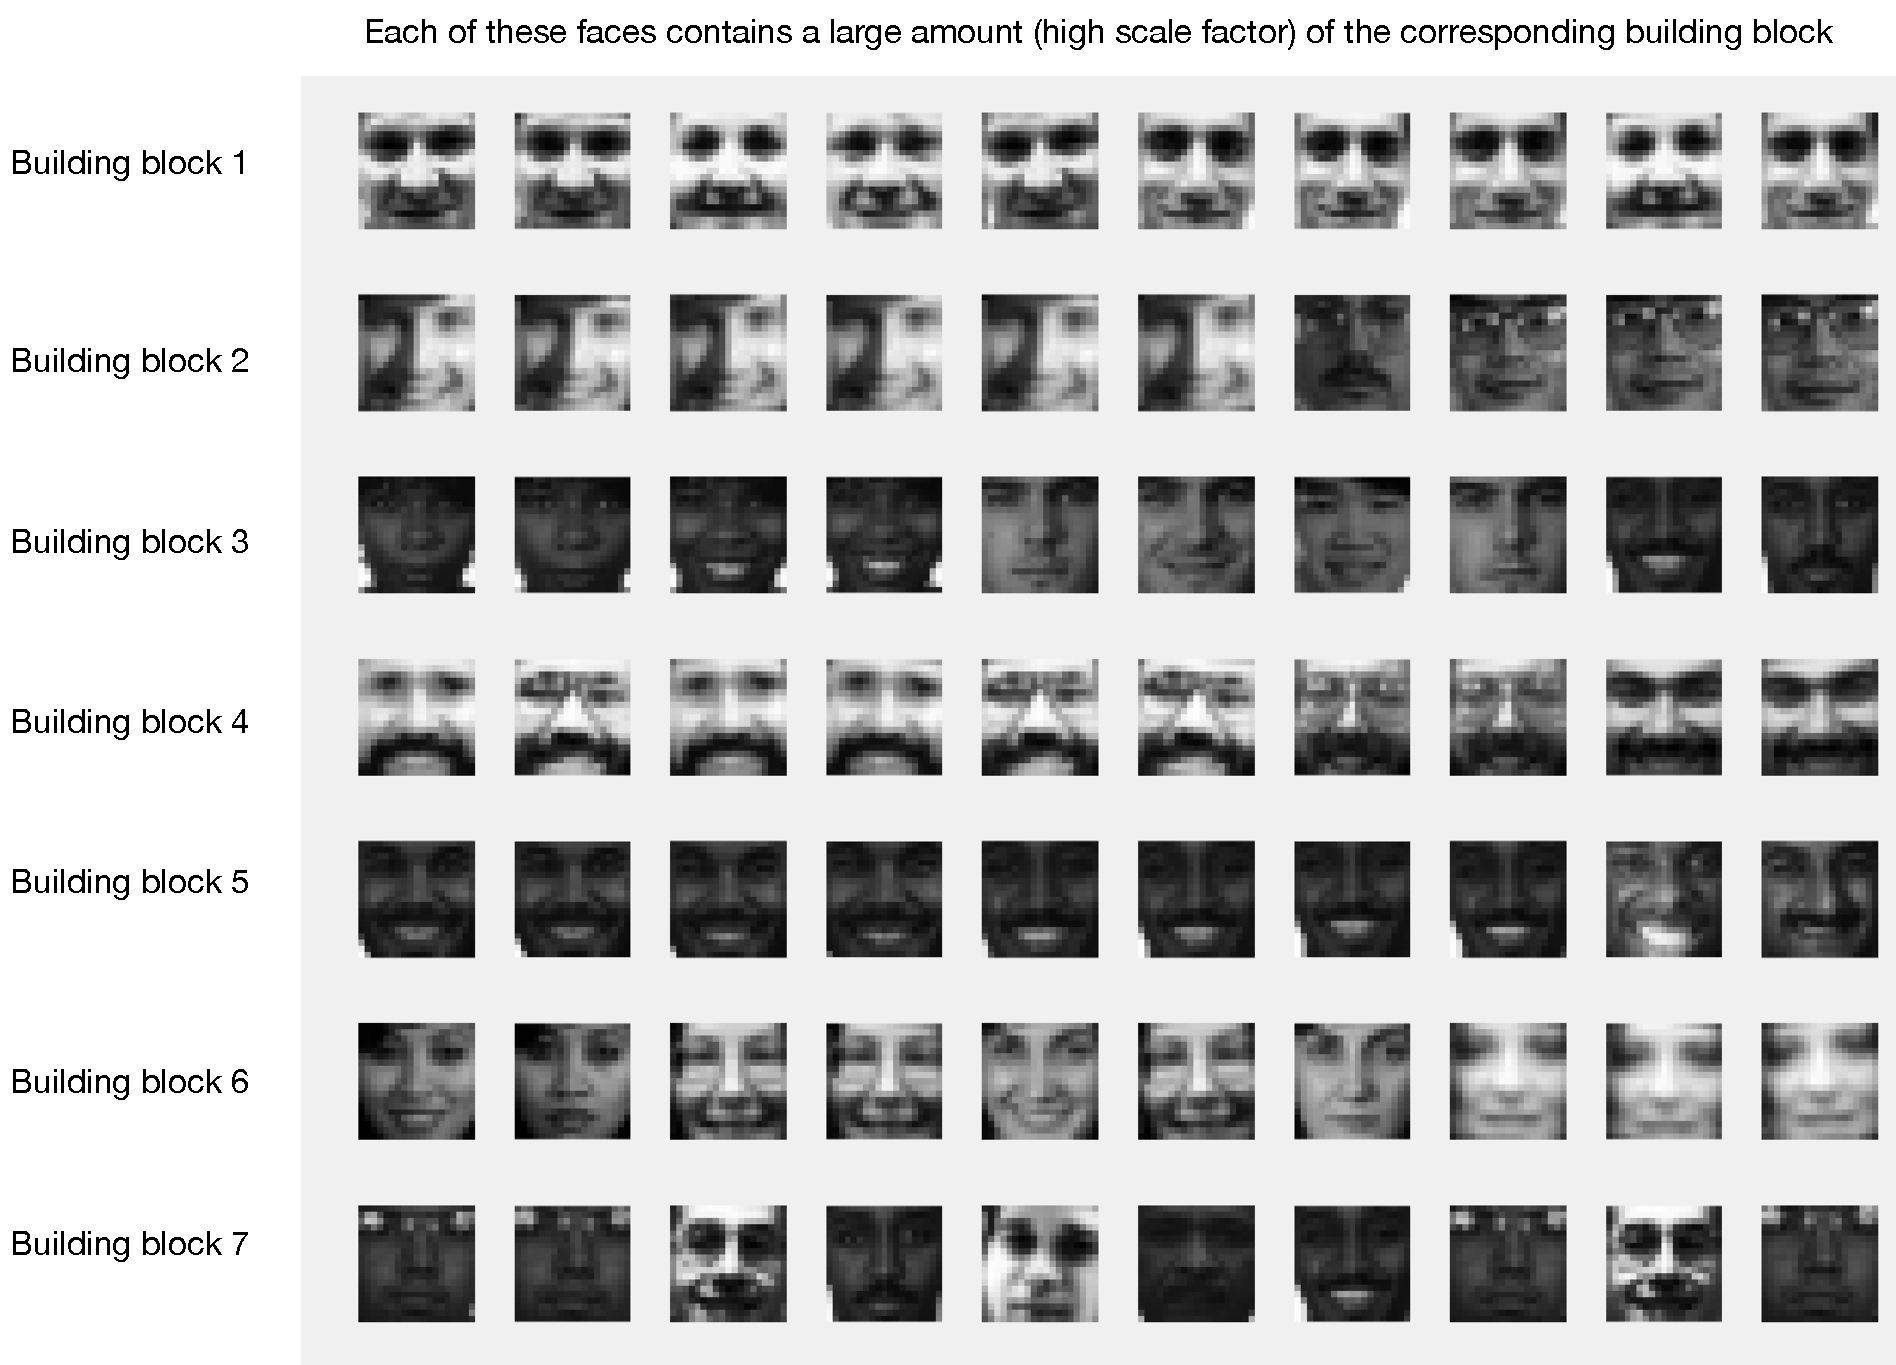
\includegraphics[width=0.8\linewidth]{FacesDay1/figs/maximumfaces}
\end{center}

\end{itemize}

\subsection{Towards an Optimal Basis [20 mins]}

\begin{prob}
\emph{In this question, we want you to think about process rather than particular techniques for solving this problem.  If you have questions on what we mean by this, let us know.}

Suppose someone has hired you as a consultant to create a method to encode 19 pixel by19 pixel images of faces (similar to the ones you just experimented with) as a sum of scaled versions of just 10 building block images.

\begin{enumerate}
\item What questions would you want to ask the person that hired you in order to do a good job on this project? (i.e., what information do you need to know?)
\item What might be some qualities of a good set of building block images?  (e.g., how would they look?  what sort of dimensions of variability would they have?)
\item What sort of data might you need to collect in order to inform the set of building blocks you will ultimately deliver (this data could be images or it could be other quantitative or qualitative data)?
\item How might you determine whether your method is working (these could be quantitative measurements or qualitative observations of your system)?
\item Are there any other steps might you want to take to complete the project?
\item We will be digging into the various dimensions of the use of facial recognition technology in society later in this module, but for now we want to get you thinking about two particular components of that.  Many face processing technologies work best on white males (e.g., check out the \href{http://gendershades.org/overview.html}{Gender Shades project}).  One possible explanation for this phenomenon is overt bias on the part of the creators of these technologies.  Instead, for the sake of this exercise, let's suppose that the differences in performance are actually the result of subtle, unconscious bias in any number of decisions that the technology creators made during the design process.  A second problem that plagues face processing algorithms is that they seem to work great when evaluated in the settings that the technology designers had in mind when they built the technology, but often work poorly when deployed in the real world.  Looking back on the steps you listed above, flag steps that might have the potential to introduce bias into your system (e.g., having your system work better on one group of people than another or having it fail in a particular use case).  It's okay if you don't know where bias might creep in, the purpose of this exercise is to get you asking questions rather than reaching conclusions.
\end{enumerate}

\end{prob}

%
%Note to John: I'm debating removing the quote below (and maybe just having it on hand in case someone asks).  I worry it might cause the debrief to be overly focused on this sone datasets, that honestly we don't really know all that much about.Paul: I agree.....
%
%It turns out one of the biggest sources of bias with respect to face processing algorithms is in the set of data used to construct and validate these algorithms.  The set of building block images we gave to you on transparencies was built using a very old (and very small by modern standards) database of faces.  in fact, the conditions under which the dataset was collected are not very well described.  Here is the relevant text from \href{https://pdfs.semanticscholar.org/f331/7b98195fe0be4acf7b450f015c1abca13ab9.pdf}{the paper that introduced this dataset}.
%
%\begin{quote}
%How do we build a comprehensive but tractable database of face and non-face patterns? For face patterns, the task at hand seems rather straight forward. We simply
%collect all the frontal views of faces we can find in mugshot databases and other image
%sources. Because we do not have access to many mugshot databases and the size of our
%mugshot databases are all fairly small, we do not encounter the problem of having to deal
%with an unmanageably large number of face  patterns. In fact, to make our set of face patterns more comprehensive, we even articially enlarged our data set by adding virtual
%examples of faces to the face database. These virtual examples are mirror images and slightly rotated versions of the original face patterns.
%
%~~~~~~~~~~~~~~-- page 70 from \href{https://pdfs.semanticscholar.org/f331/7b98195fe0be4acf7b450f015c1abca13ab9.pdf}{Learning and Example Selection for Object and Pattern Detection}
%\end{quote}
%
%We'll be using this quote along with your other experiences in this activity as fodder for our course wide debrief.